\chapter{O Método de Elementos Discretos} \label{ch:discrete_element_method}

\alert{Descrever aqui as características básicas e gerais que o \DEM{} possui}

\alert{Falar das forças externas, que são fundamentais para algumas das simulações}

\alert{Mostrar os principais aspectos do algoritmo e passar por cada um deles, detalhando}

\alert{Falar do critério de parada}

O Método de Elementos Discretos (\DEM{}\footnote{Do inglês, \textit{Discrete Element Method}.}) refere-se a uma família de métodos numéricos aplicados na simulação de sistemas de partículas. Esses métodos compartilham diversas características entre si, como o monitoramento da vizinhança de cada partícula, o cálculo explícito das variáveis do problema a partir de seus valores nos instantes anteriores, dentre outras.

Este capítulo é dedicado à apresentação e à explicação dessas características. São apresentados o funcionamento geral de um algoritmo \DEM{}, o procedimento de solução das equações do problema e as principais etapas do método.

\alert{Talvez descrever melhor o que há em cada seção}

\section{Características Gerais do Método}

Segundo \citeonline[p. 1]{bib:bicanic2007}, o \DEM{} constitui-se de técnicas de modelagem computacional indicadas para a simulação do comportamento dinâmico de conjuntos de partículas de geometria arbitrária sujeitas a restrições de contato variantes no tempo.

Conforme a definição apresentada por \apudonline{bib:cundall1989}{bib:bicanic2007}, métodos de elementos discretos são métodos computacionais que:
\begin{alineas}
	\item consideram deslocamentos e rotações finitos de corpos discretos;
	\item reconhecem novos contatos automaticamente à medida que a simulação progride.
\end{alineas}

Cada partícula é considerada um corpo rígido com seis graus de liberdade: três translações e três rotações, e está sujeita às equações diferenciais de movimento descritas na \autoref{sec:equations_of_motion}. O processo de simulação consiste na solução dessas equações. 

Em um sistema, porém, os elementos interagem entre si, e as forças e os torques atuantes sobre eles dependem dessas interações. Sendo assim, é necessário o \textit{monitoramento das vizinhanças}, isto é, o método deve sempre determinar quais são os pares de elementos que interagem em cada passo de tempo. Dentre os algoritmos disponíveis, destacam-se o algoritmo de Verlet, dedicado a partículas esféricas, o algoritmo \textit{link cell} e o algoritmo \textit{lattice}. \alert{São esses mesmo que considero depois?}

Os elementos da simulação ainda podem pertencer a \textit{tipos} distintos. Por exemplo, é possível distinguirem-se \textit{partículas}, elementos cujas equações de movimento precisam ser resolvidas, de \textit{elementos de contorno}, que têm seu estado conhecido já na etapa de inicialização do algoritmo. Além dos elementos de contorno, outras \textit{condições de contorno} podem ser aplicadas ao sistema, como restrições de movimento, paredes reflexivas e condição de repetição.

De acordo com \citeonline[p. 2]{bib:bicanic2007}, existem diversas metodologias para a simulação com elementos discretos, sendo que as variações ocorrem:
\begin{alineas}
	\item nos algoritmos de detecção de contatos;
	\item nas formulações para as interações;
	\item nas condições de contorno;
	\item na consideração de modelos de fratura, fragmentação ou aglutinação;
	\item nos métodos de integração das equações;
	\item nos algoritmos de monitoramento de vizinhanças.
\end{alineas}

\subsection{Discretização Temporal}

Como é recorrente em métodos de simulação numérica, o \DEM{} conta com a discretização do tempo para a solução das equações de movimento. Para o intervalo de simulação \(\interval{\initialInstant}{\finalInstant}\), sendo \(\initialInstant\) o instante inicial e \(\finalInstant\), o final, uma discretização temporal é um conjunto \(\set{t_0, t_1, \dotsc, t_{\numberOfTimesteps}}\) tal que
\begin{equation*}
	\initialInstant = \instant[0] < \instant[1] < \dotsb < \instant[\numberOfTimesteps - 1] < \instant[\numberOfTimesteps] = \finalInstant.
\end{equation*}

O valor \(\numberOfTimesteps\) é o número de passos de tempo da simulação. Um passo de tempo é o período compreendido entre dois instantes consecutivos da discretização. A duração do \(n\)-ésimo passo de tempo é dada então por
\begin{equation*}
	\Dt[n] \eqdef \instant[n] - \instant[n-1],
\end{equation*}
e escreve-se \(\Dt\) no caso em que os passos de tempo têm todos a mesma duração.

Com isso, o objetivo do Método de Elementos Discretos torna-se obter a solução para as coordenadas das partículas no tempo discretizado.

\subsection{Solução das Equações}

A solução das equações governantes do sistema é feita conforme explicado na \autoref{subsec:motion_equations_solution} utilizando algoritmos de integração como o algoritmo de Gear, descrito na \autoref{sec:gear_integration_scheme}.

Uma característica dos métodos de elementos discretos é serem métodos explícitos, ou seja, o estado do sistema de partículas no instante \(\instant[n]\) é calculado a partir do estado em \(\instant[n-1]\) que se supõe ser conhecido. Isso é evidente no algoritmo de Gear.

De acordo com \citeonline{bib:computational_granular_dynamics}, a solução das equações pode ser dividida em quatro etapas, sendo elas:

% \begin{enumdesc}
% 	\item[Determinação da Vizinhança:] Nessa etapa, a vizinhança de cada partícula do sistema é construída (no primeiro instante) ou atualizada (em instantes posteriores da simulação). O objetivo é limitar a quantidade de interações avaliadas no passo de tempo. 
% 	\item[Predição:] Nesse passo, o estado do sistema no instante \(\instant[n]\) é predito em função do estado em \(\instant[n-1]\). Essa predição é feita por métodos de extrapolação, como explicado na \autoref{subsec:prediction}. \label{item:DEM_prediction}
% 	\item[Interação:] A partir do estado predito do sistema, são computadas as interações entre cada partícula e os elementos de sua vizinhança. \label{item:DEM_interaction}
% 	\item[Correção:] Na etapa de correção, o estado do sistema no instante \(\instant[n]\) é corrigido em função das interações calculadas na etapa \ref{item:DEM_interaction} e das equações governantes do problema, como apresentado na \autoref{subsec:correction}. Embora esse processo não seja exato, o DEM considera o estado corrigido como a solução do problema para o instante \(\instant[n]\). \label{item:DEM_correction}
% \end{enumdesc}
\begin{enumerate}
	\item \textit{Determinação da Vizinhança:} Nessa etapa, a vizinhança de cada partícula do sistema é construída (no início da simulação) ou atualizada (em instantes posteriores) com o intuito de limitar a quantidade de interações avaliadas no passo de tempo. \label{item:DEM_neighborhood}
	\item \textit{Predição:} Nesse passo, o estado do sistema no instante \(\instant[n]\) é predito em função do estado em \(\instant[n-1]\) por meio de métodos de extrapolação, como explicado na \autoref{subsec:prediction}. \label{item:DEM_prediction}
	\item \textit{Interação:} A partir do estado predito do sistema, são computadas as interações entre cada partícula e os elementos de sua vizinhança. \label{item:DEM_interaction}
	\item \textit{Correção:} Na etapa de correção, o estado do sistema no instante \(\instant[n]\) é corrigido em função das interações calculadas na etapa \ref{item:DEM_interaction} e das equações governantes do problema, como apresentado na \autoref{subsec:correction}. Embora esse processo não seja exato, o DEM considera o estado corrigido como a solução do problema para o instante \(\instant[n]\). \label{item:DEM_correction}
\end{enumerate}

Os passos \ref{item:DEM_prediction}, \ref{item:DEM_interaction} e \ref{item:DEM_correction} são específicos do algoritmo de Gear, podendo mudar se forem adotados outros métodos.

Para a determinação da vizinhança no passo \ref{item:DEM_neighborhood}, são usados algoritmos de monitoramento de vizinhança, como explicado na \autoref{sec:neighborhood}. O objetivo desta seção é, assim, apresentar os passos \ref{item:DEM_prediction}, \ref{item:DEM_interaction} e \ref{item:DEM_correction}, mostrando a aplicação dos conceitos apresentados no \autoref{ch:mathematical_model} aos sistemas de partículas.

% \alert{é estranho colocar a vizinhança antes. Três motivos por que isso é feito: 1) a referência faz; 2) o passo de tempo que usamos é pequeno; 3) permite uma fácil alteração do algoritmo de integração da equação}

Pode ser feita uma distinção entre o caso de partículas com geometria arbitrária, em que é necessário monitorar-se a orientação das partículas, e o de partículas esféricas, situação em que é possível aplicarem-se simplificações.

\subsubsection*{Caso Geral}

No caso de partículas quaisquer, o algoritmo de Gear precisa levar em consideração as parametrizações para as orientações das partículas.

Sendo \(\instant[n]\) o instante de interesse e \(\instant[n-1]\), o instante anterior em que o sistema é conhecido, as posições e as orientações das partículas podem ser previstas como na equação \eqref{eq:prediction}. Escolhida uma ordem de extrapolação \(\taylorOrder\), e definido o conjunto \(\particleSet\) de partículas do sistema, calculam-se
\begin{equation*}
	\def\arraystretch{1.5}
	\begin{array}{c}
		\drvec{\taylorOrder}{\positionipr}\pqty{\instant[n]} = \extrapolationMatrix{\taylorOrder}[\Dt[n]]\cdot\drvec{\taylorOrder}{\positioni}\pqty{\instant[n-1]} \\
		\drvec{\taylorOrder}{\orientationipr}\pqty{\instant[n]} = \extrapolationMatrix{\taylorOrder}[\Dt[n]]\cdot\drvec{\taylorOrder}{\orientationi}\pqty{\instant[n-1]} \\
	\end{array}, \quad \particlei \in \particleSet,
\end{equation*}
em que \(\extrapolationMatrix{\taylorOrder}[\Dt[n]]\) é a matriz de extrapolação por expansão de Taylor de ordem \(\taylorOrder\) calculada com o passo de tempo \(\Dt[n]\), como indicada na \autoref{subsec:prediction}.

A vizinhança de uma partícula, como explicado na \autoref{sec:neighborhood}, é o conjunto de todas as entidades da simulação com as quais ela interage. A vizinhança da \(i\)-ésima partícula do sistema é denotada por \(\neighborhoodi\) \alert{Verificar se essas coisas já não foram ditas antes com a mudança das seções.}. Cada elemento \(\elementj\) da vizinhança de \(\particlei\) contribui para a força \(\forcei\) e o torque \(\torquei\) resultantes sobre a mesma com parcelas \(\forceji\) e \(\torqueji\) que são, por hipótese, dependentes apenas do par \(\orderedPair{\particlei}{\elementj}\), isto é,
\begin{equation*}
	\def\arraystretch{1.5}
	\begin{array}{c}
		\displaystyle \forceji \equiv \forceji\pqty{\particlei, \elementj} \\
		\displaystyle \torqueji \equiv \torqueji\pqty{\particlei, \elementj} \\
	\end{array}, \quad \particlei \in \particleSet, \elementj \in \neighborhoodi.
\end{equation*}

Mais ainda, a partícula \(i\) pode sofrer com forças e torques provocados por entidades externas ao sistema, como forças de campo, cujas resultantes são dadas por
\begin{equation*}
	\def\arraystretch{1.5}
	\begin{array}{c}
		\external\forcei \equiv \external\forcei\pqty{\particlei} \\
		\external\torquei \equiv \external\torquei\pqty{\particlei} \\
	\end{array}, \quad \particlei \in \particleSet.
\end{equation*}
 
Com isso, obtêm-se os vetores resultantes de acordo com o princípio da superposição dado pelas equações \eqref{eq:superposition_translation} e \eqref{eq:superposition_rotation}:
\begin{equation*}
	\def\arraystretch{1.5}
	\begin{array}{c}
		\resultingForcei = \dsum_{\elementj\in\neighborhoodi}\forceji + \external\forcei\\
		\resultingTorquei = \dsum_{\elementj\in\neighborhoodi}\torqueji + \external\torquei
	\end{array}, \quad \particlei\in\particleSet.
\end{equation*}

A cada um dos graus de liberdade da partícula é associada uma equação que determina seu comportamento, e o algoritmo de Gear baseia-se nisso para executar a etapa de correção. As equações de movimento \eqref{eq:motion_first} e \eqref{eq:diff_equation_orientation_parametrization}, então, são utilizadas para se corrigirem as derivadas de segunda ordem da posição e da orientação das partículas:
\begin{equation*}
	\def\arraystretch{1.5}
	\begin{array}{c}
		\displaystyle \accelerationicorr =  \dfrac{1}{\massi}\cdot \forcei \\
		\displaystyle \dorientationicorr{2} = \eqFor{\orientationScalar}\pqty{\torquei, \orientationipr, \dorientationipr{1}}
	\end{array}, \quad \particlei \in \particleSet,
\end{equation*}
sendo que \(\eqFor{\orientationScalar}\) depende da parametrização escolhida para a orientação.

Definem-se, então, os erros
\begin{equation*}
	\def\arraystretch{1.5}
	\begin{array}{c}
		\Delta \accelerationi\pqty{\instant[n]} = \accelerationicorr\pqty{\instant[n]} - \accelerationipr\pqty{\instant[n]} \\
		\Delta \dorientationi{2}\pqty{\instant[n]} = \dorientationicorr{2}\pqty{\instant[n]} - \dorientationipr{2}\pqty{\instant[n]} \\
	\end{array}, \quad \particlei\in\particleSet.
\end{equation*}

Por fim, resta executar a correção nos vetores de derivadas. Tanto para a translação quanto para a rotação, a equação diferencial é de ordem \(\eqOrder = 2\), e isso, juntamente com a ordem de extrapolação \(\taylorOrder\), determina as constantes de correção. Com isso, utiliza-se a equação \eqref{eq:correction_simplified} para se escrever	
\begin{equation*}
	\def\arraystretch{1.5}
	\begin{array}{l}
		\drvec{\taylorOrder}{\positionicorr}\pqty{\instant[n]} = \drvec{\taylorOrder}{\positionipr}\pqty{\instant[n]} + \correctorConstantVector{\taylorOrder}{2}\cdot\dfrac{\Dt[n]^2}{2}\Delta \accelerationi\pqty{\instant[n]} \\
		\drvec{\taylorOrder}{\orientationicorr}\pqty{\instant[n]} = \drvec{\taylorOrder}{\orientationipr}\pqty{\instant[n]} + \correctorConstantVector{\taylorOrder}{2}\cdot\dfrac{\Dt[n]^2}{2}\Delta \dorientationi{2}\pqty{\instant[n]}
	\end{array}, \quad \particlei\in\particleSet.
\end{equation*}

Dessa forma, estão calculadas a posição, a orientação e as suas derivadas, e o instante de tempo \(\instant[n]\) é considerado solucionado.

\subsubsection*{Partículas Esféricas}

Para partículas esféricas, as equações de movimento assumem uma forma mais simples, conforme mostrado na \autoref{subsubsec:rotation_of_spherical_particles}. 

Novamente, o algoritmo inicia com a escolha da ordem de derivação \(\taylorOrder\) para a predição conforme a equação \eqref{eq:prediction}. Dessa vez, porém, a velocidade angular é prevista com uma ordem a menos que a posição.
\begin{equation*}
	\def\arraystretch{1.5}
	\begin{array}{c}
		\drvec{\taylorOrder}{\positionipr}\pqty{\instant[n]} = \extrapolationMatrix{\taylorOrder}[\Dt[n]]\cdot\drvec{\taylorOrder}{\positioni}\pqty{\instant[n-1]} \\
		\drvec{\taylorOrder-1}{\angularVelocityipr}\pqty{\instant[n]} = \extrapolationMatrix{\taylorOrder-1}[\Dt[n]]\cdot\drvec{\taylorOrder-1}{\angularVelocityi}\pqty{\instant[n-1]} \\
	\end{array}, \quad \particlei\in\particleSet.
\end{equation*}

O cálculo de forças e torques se dá de maneira idêntica ao caso geral, isto é,
\begin{equation*}
	\def\arraystretch{1.5}
	\begin{array}{c}
		\resultingForcei = \dsum_{\elementj\in\neighborhoodi}\forceji\pqty{\particlei, \elementj} + \external\forcei\pqty{\particlei}\\
		\resultingTorquei = \dsum_{\elementj\in\neighborhoodi}\torqueji\pqty{\particlei, \elementj} + \external\torquei\pqty{\particlei}
	\end{array}, \quad \particlei\in\particleSet.
\end{equation*}

E, como no caso geral, o valor corrigido para a aceleração advém da equação \eqref{eq:motion_first}:
\begin{equation*}
	\accelerationicorr\pqty{\instant[n]} = \dfrac{1}{\massi}\cdot\resultingForcei\pqty{\instant[n]}, \quad\particlei\in\particleSet.
\end{equation*}

Já para a aceleração angular, usa-se a equação de movimento rotacional simplificada para o caso de esferas \eqref{eq:rotation_spherical_particle}, obtendo-se, para cada \(\particlei\in\particleSet\),
\begin{equation*}
	\dangularVelocityicorr{1}\pqty{\instant[n]} = \dfrac{1}{\momentOfInertiai}\cdot\resultingTorquei\pqty{\instant[n]}
\end{equation*}

Com isso, os erros são dados por
\begin{equation*}
	\def\arraystretch{1.5}
	\begin{array}{c}
		\Delta \accelerationi\pqty{\instant[n]} = \accelerationicorr\pqty{\instant[n]} - \accelerationipr\pqty{\instant[n]} \\
		\Delta \dangularVelocityi{1}\pqty{\instant[n]} = \dangularVelocityicorr{1}\pqty{\instant[n]} - \dangularVelocityipr{1}\pqty{\instant[n]} \\
	\end{array}, \quad\particlei\in\particleSet.
\end{equation*}

E, finalmente, são corrigidos os vetores de derivadas conforme a equação \eqref{eq:correction_simplified}. Para a translação, a equação diferencial é de ordem \(\eqOrder = 2\), e então
\begin{equation*}
	\drvec{\taylorOrder}{\positionicorr}\pqty{\instant[n]} = \drvecipr{\taylorOrder}{\position}\pqty{\instant[n]} + \correctorConstantVector{\taylorOrder}{2}\cdot\dfrac{\Dt[n]^2}{2}\Delta \accelerationi\pqty{\instant[n]}, \quad\particlei\in\particleSet.
\end{equation*}

A velocidade angular, por sua vez, está sujeita a uma equação diferencial de primeira ordem. O vetor de coeficientes \(\correctorConstantVector{\taylorOrder-1}{1}\), portanto, deve ser calculado para \(\eqOrder=1\). Nessas condições, o vetor de derivadas da velocidade angular fica
\begin{equation*}
		\drvec{\taylorOrder}{\angularVelocityicorr}\pqty{\instant[n]} = \drvec{\taylorOrder}{\angularVelocityipr}\pqty{\instant[n]} + \correctorConstantVector{\taylorOrder-1}{1}\cdot\Dt[n]\cdot\Delta \dangularVelocityi{1}\pqty{\instant[n]}, \quad\particlei\in\particleSet.
\end{equation*}

\alert{continuar}

\alert{Mostrar isso em forma de fluxograma e de pseudocódigo}

\begin{lstlisting}[style=pseudocode]
para cada partícula $\particlei \in \particleSet$
	para cada vizinho $\elementj \in \neighborhoodi$
		calcular \forceji
		calcular \torqueji
\end{lstlisting}

\subsection{Elementos da Simulação}

Toda simulação possui um \textit{conjunto universo} \(\universeSet\) que consiste em todas as entidades consideradas pelo algoritmo: elementos, fluidos, campos de força, entre outras. Nos métodos de elementos discretos, os corpos rígidos pertencentes ao conjunto universo são agrupados no \textit{conjunto de elementos} \(\elementSet\). Por fim, é possível dividir-se o conjunto de elementos em um \textit{conjunto de partículas} \(\particleSet\) e um \textit{conjunto de elementos de contorno} \(\boundarySet\).

O conjunto de partículas é o conjunto de todos os elementos para os quais as equações de movimento devem ser resolvidas. Essa resolução é feita de acordo com os algoritmos de integração. 

Os elementos de contorno, por outro lado, são elementos cujos estados já são conhecidos como funções explícitas do tempo desde a etapa de inicialização. Exemplo disso são os elementos fixos, cujas coordenadas são sempre iguais às coordenadas iniciais.

\alert{Continuar}

\subsubsection{Tipos de Elementos}
\subsubsection{Geometria}

A geometria dos elementos de um sistema de um sistema de partículas é \alert{o quê?}

\subsection{Algoritmo Geral do \DEM{}} \label{sec:dem_algorithm}

\section{Etapas do Algoritmo}
\subsection{Inicialização do Sistema de Partículas}

A primeira etapa em uma simulação \DEM{} consiste na inicialização do sistema de partículas. Essa inicialização consiste em se definir o ambiente da simulação e se construírem todos os elementos necessários.

\alert{Falar das condições iniciais}

\subsection{Laço da Simulação}
\alert{É esse mesmo o nome? Falar aqui sobre o ciclo previsão - cálculo de forças - correção}

\subsection{Exportação de Dados}

\subsection{Condição de Parada}

\subsection{Finalização}\alert{Talvez essa seja a seção mais inútil. Talvez excluí-la. Mas falar que o último timestep pode ser usado como inicialização para outras simulações}

\section{Monitoramento da Vizinhança} \label{sec:neighborhood}
\alert{Dividir em vizinhança global, local e contato: em uma, o domínio é dividido em regiões. Partículas só podem colidir com as que estão na mesma região ou em regiões vizinhas à sua. Depois, os vizinhos locais: Define-se, em torno da partícula, um volume envolvente. Duas partículas só podem colidir se houver contato entre seus volumes envolventes. Por fim, avalia-se o contato efetivamente, levando em conta a geometria das partículas.}

\alert{Falar dos métodos de busca de vizinhos}

\alert{Verificar se já não falei dos custos do cálculo das forças} Segundo \citeonline[p. 26]{bib:computational_granular_dynamics}, o maior custo computacional em uma simulação de elementos discretos está associado à avaliação das forças atuantes sobre as partícula em cada passo de tempo. Em um sistema de \(\numberOfParticles\) elementos, e com a simplificação de que a interação de cada par interagente é independente dos demais, cada partícula pode interagir com até \(\numberOfParticles-1\) outros elementos. Isso resulta em um total de
\begin{equation*}
	\numberOfParticles\cdot\pqty{\numberOfParticles-1}
\end{equation*}
interações computadas a cada passo de tempo.

\alert{Usei as palavras ``interação'' e ``cada'' diversas vezes nesse parágrafo...}

Essa quantidade de interações, porém, limita o número de partículas e de passos de tempo aplicáveis. Buscam-se, então, métodos mais eficientes para o monitoramento da vizinhança de cada elemento. 

\alert{Onde escrever a parte a seguir: ?}

A vizinhança de uma partícula \(\particlei\) é o conjunto \(\neighborhoodi\) de todos os elementos da simulação com os quais a partícula pode interagir. Sendo \(\particleSet\) o conjunto de todas as partículas do sistema, pode-se definir
\begin{equation*}
	\neighborhoodi = \particleSet \setminus \Bqty{\particlei}.
\end{equation*}

Entretanto essa definição resulta em tempos de simulação elevados.

Uma simples consideração, a terceira lei de Newton, reduz pela metade a quantidade de interações avaliadas. \alert{Continuar aqui}

\subsection{Terceira Lei de Newton}

Dadas duas partículas \(\particlei\) e \(\particlej\), a terceira lei de Newton estabelece que à força \(\forceij\) que a partícula \(i\) aplica sobre a \(j\) corresponde uma reação \(\forceji\) que satisfaz
\begin{equation*}
	\forceji = -\forceij.
\end{equation*}
Esse princípio possui duas consequências. A primeira, que, se \(\particlej\) está na vizinhança de \(\particlei\), então \(\particlei\) está, necessariamente, na vizinhança de \(\particlej\).

A segunda é que a força de interação entre \(i\) e \(j\) precisa ser computada apenas uma vez.

\alert{Eu ficaria mais feliz se a primeira fosse representada por uma figura ou uma equação para a vizinhança, mostrando a vizinhança explícita e a vizinhança implícita.}

\subsection{Algoritmo de Verlet}

De acordo com \citeonline{bib:computational_granular_dynamics}, o algoritmo de Verlet é um método de monitoramento de vizinhanças que fundamenta-se em duas considerações:
\begin{itemize}
	\item Uma partícula só pode colidir com partículas que estejam próximas a ela.
	\item \alert{Caso as partículas não se movam o suficiente, a vizinhança é constante}
\end{itemize}

Nesse método, considera-se que duas partículas são vizinhas se a menor distância entre suas superfícies for menor que uma constante arbitrada \(\verletDistance\) denominada de \textit{distância de Verlet}.

\begin{figure}[h]
	\caption{Representação da vizinhança de partículas esféricas no algoritmo de Verlet. Duas partículas são vizinhas se a distância entre suas superfícies for menor que a distância de Verlet \(\verletDistance\)}
	% \vspace{-0.5cm}
	\begin{center}
		\alert{Colocar imagem representando a distância de Verlet. Mostrar três pares de partículas: não vizinhas, caso extremo em que são quase vizinhas e vizinhas}
		% 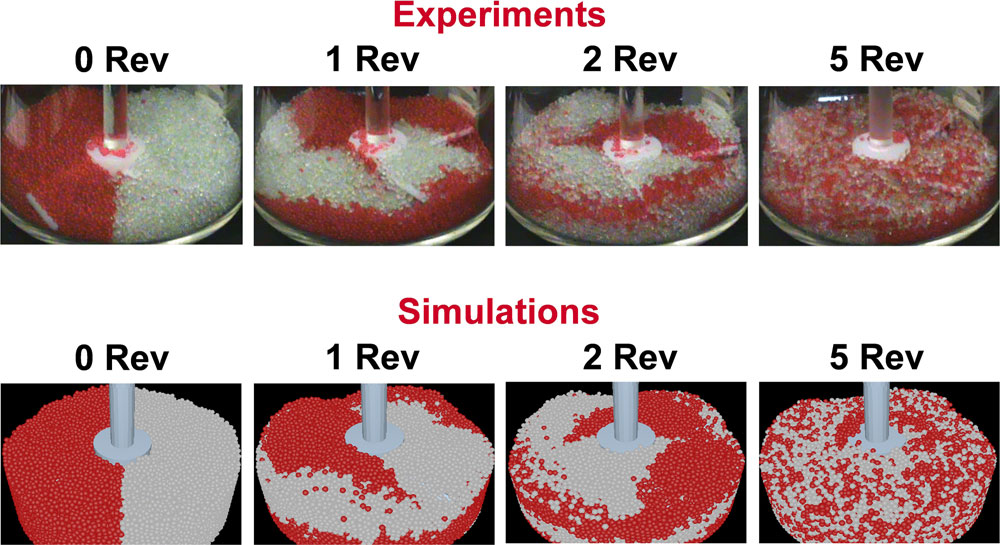
\includegraphics[width=0.65\textwidth]{images/introduction/drug_production.png}
	\end{center}
	% {\centerline{\includegraphics[scale=#2]{#1}}}
	% \vspace{-0.2cm}
	\label{fig:verlet_distance}
	\source{\alert{Citar fonte}}
	% \vspace{-1cm}
\end{figure}

Para partículas esféricas \(\particlei\) e \(\particlej\), a condição de vizinhança se escreve como
\begin{equation*}
	\norm{\positioni - \positionj} < \radiusi + \radiusj + \verletDistance,
\end{equation*}
como indicado na figura \ref{fig:verlet_distance}, e então a vizinhança da partícula \(i\) é o conjunto
\begin{equation*}
	\neighborhoodi = \set{\particlej \suchThat \alert{}}
\end{equation*}

\alert{Mostrar o conjunto vizinhança e dizer que, para o algoritmo de Verlet, esse conjunto é denominado de lista de Verlet}
\alert{Definir o deslocamento de Verlet como a distância \(\verletPosition\) entre a partícula e a sua posição quando a última lista de Verlet foi construída}

% Com isso, no instante \(\instant[n-1]\), a vizinhança da \(i\)-ésima partícula é o conjunto
% \begin{equation*}
% 	\neighborhoodi\pqty{\instant[n-1]} = \left\lbrace\particlej \,\suchThat\, \distanceij\pqty{\instant[n-1]} < \radiusi + \radiusj + \verletDistance\right\rbrace,
% \end{equation*}
% em que \(\distanceij\) é a distância entre os centros das partículas \(i\) e \(j\).

Ao longo da simulação, porém, a movimentação das partículas faz  com que sua vizinhança se altere, e então é necessário reconstruir as listas de Verlet. O critério para a reconstrução das listas leva em consideração a situação extrema

\alert{continuar}

O algoritmo de Verlet, embora bastante eficiente para partículas esféricas \alert{Falar ainda que há como otimizar isso}

\subsection{Algoritmo \textit{link cell}}
\subsection{Algoritmo \textit{lattice}}

\section{Identificação de Contatos}

\section{Limitação do Passo de Tempo}

\alert{Ver \citeonline{bib:cundall1979} e \citeonline{bib:gomes2014}}

\alert{Explicar que o passo de tempo deve ser menor que um limite. Ver se essa seção é mesmo necessária.}

\section{Condições de Contorno e Restrições} \label{sec:boundary_condition}

\alert{Falar das condições de contorno: partículas com movimento pré-determinado, condição de repetição e de reflexão (parede que reflete a partícula)}

\section{Outros Aspectos do Método}
\alert{Considerar, principalmente, \citeonline{bib:bicanic2007}. Essa seção deve falar que existem o estudo de fratura e fragmentação, abordagem para corpos deformáveis e esquemas de variação do passo de tempo}
\alert{Falar da paralelização}

\section{Acoplamento com Outros Métodos}
\alert{Falar aqui como o \DEM{} pode ser acoplado com CFD e FEM}